정렬(sorting)은 어떤 배열의 값들을 작은 수부터 큰 수 또는 큰 수부터 작은 수의 순서로 나열하는 것을 말한다. 이 장에서는 총 7가지 정렬 알고리즘과 정렬 기준 설정에 대해 배울 것이다.

\section{비교 기반 정렬 알고리즘}
비교 기반 정렬 알고리즘은 어떤 두 수를 비교해 얻은 결과만을 이용해 정렬하는 알고리즘이다. 다른 말로, 배열 $arr$에 속하는 어떤 두 수 $x, y$를 비교해 더 작은 수가 앞에 와야 함을 이용해 정렬하는 것이다.

이러한 비교 기반 정렬 알고리즘의 특징은 시간복잡도의 상한이 $O(N \log N)$이라는 것이다. 그 이유는 $N$개의 데이터에서 존재할 수 있는 모든 초기 데이터가 $N!$가지인데, 적절한 한 번의 비교를 통해 가능한 경우의 수를 절반으로 줄일 수 있기 때문에 최소 연산 횟수는 $O(\log N!)$로 정해져 있기 때문이다(스털링 근사에 의해 $O(N!)=O(N \log N)$이 된다). 

이 절에서는 총 다섯 종류의 비교 기반 정렬 알고리즘을 다룬다. 앞 3개는 평균 시간복잡도가 $O(N^2)$인 알고리즘, 뒤 2개는 평균 시간복잡도가 $O(N \log N)$인 알고리즘이다. 비교 기반 정렬 알고리즘은 모두 중요하므로 주의 깊게 보도록 하자.

\subsection{버블 정렬}
버블 정렬은 인접한 두 수를 비교해 큰 수가 앞에 있으면 뒤집는 과정을 반복함으로써 정렬하는 방식이다. 정확히 말하면 $1 \leq i < N$인 모든 $i$에 대해 $i$번째 수와 $i+1$번째 수의 크기 순서가 반대이면 $i$번째 수와 $i+1$번째 수를 뒤집는 과정을 정렬될 때까지 반복하는 것이다. \Cref{code: bubble}에 구현 코드가 있다.

\begin{code} \label{code: bubble}
버블 정렬 구현 코드
\begin{lstlisting}
#include <bits/stdc++.h>
using namespace std;

int n, arr[1010];

bool check() {
    for (int i = 1; i < n; i++) {
        if (arr[i] > arr[i + 1]) return true;
    }
    return false;
}

int main() {
    cin >> n;
    for (int i = 1; i <= n; i++) cin >> arr[i];

    while (check()) {
        for (int i = 1; i < n; i++) {
            if (arr[i] > arr[i + 1]) swap(arr[i], arr[i + 1]);
        }
    }

    for (int i = 1; i <= n; i++) cout << arr[i] << " ";
    return 0;
}
\end{lstlisting}
\end{code}

버블 정렬의 시간복잡도는 어떻게 될까? 뒤집는 과정이 반복되는 횟수에 $N$을 곱한 것이 시간복잡도가 될 것이다. 그렇다면 뒤집는 과정은 얼마나 많이 반복될까? 수학적으로 $N$번 이하임을 증명할 수 있다. 즉, 버블 정렬의 시간복잡도는 $O(N^2)$이다. 증명은 \Cref{pb: bubble-pf}을 참고하라.

버블 정렬의 교환 횟수는 어떻게 될까? 한 번 교환할 때마다 $i<j$이고 $arr[i]>arr[j]$인 순서쌍 $(i, j)$의 개수가 하나씩 줄어든다는 것은 자명한 사실이다. 즉, 어떤 배열 $arr$에 대해 $i<j$이고 $arr[i]>arr[j]$인 순서쌍 $(i, j)$의 개수로 정의되는 \textit{Inversion Count}가 버블 정렬의 교환 횟수가 된다. \textit{Inversion Count}를 구하는 문제를 \Cref{pb: inversion-square}에서 풀어보라.

\subsection{삽입 정렬}
삽입 정렬은 앞에서부터 정렬해나가는 방식으로 $x$번째까지 정렬되어 있을 때 $x+1$번째를 자신보다 작은 수가 나올 때까지 앞으로 한 칸씩 옮기며 정렬하는 방식이다. 이 방법을 사용했을 때 정렬이 됨은 자명하게 확인할 수 있다. \Cref{code: insertion}를 보라.

\begin{code} \label{code: insertion}
삽입 정렬 구현 코드
\begin{lstlisting}
#include <bits/stdc++.h>
using namespace std;

int n, arr[1010];

int main() {
    cin >> n;
    for (int i = 1; i <= n; i++) cin >> arr[i];

    for (int i = 1; i <= n; i++) {
        for (int j = i; j >= 2; j--) {
            if (arr[j] < arr[j - 1]) swap(arr[j], arr[j - 1]);
            else break;
        }
    }

    for (int i = 1; i <= n; i++) cout << arr[i] << " ";
    return 0;
}
\end{lstlisting}
\end{code}

삽입 정렬의 재미있는 특징은 거의 정렬되어 있다면 빠른 시간에 완료된다는 것이다. 왜냐하면 $x$번째 수 앞에 있는 수들 중 $x$번째 수보다 큰 수의 개수와 교환 횟수가 동일하기 때문이다($N=5$일 때 배열 $1, 3, 5, 4, 2$와 $5, 4, 3, 2, 1$의 교환 횟수를 비교해 확인해보라). 이러한 특징은 전체 배열이 거의 정렬되었을 때 의도적으로 삽입 정렬을 사용하는 하이브리드 정렬에 자주 사용된다. 하지만 여전히 시간복잡도는 $O(N^2)$이다. 완전히 역순인 최악의 경우에는 교환 횟수가 $N(N-1)/2$이기 때문이다.

\subsection{선택 정렬}
선택 정렬은 배열에서 최솟값을 찾고 그 수를 제일 앞으로 보내는 과정을 반복함으로써 정렬하는 방식이다. 당연히 $k$개의 수를 앞으로 보냈다면 $k+1$번째 수부터 최솟값을 찾아야 한다. \Cref{code: selection}을 보라.

\begin{code} \label{code: selection}
선택 정렬 구현 코드
\begin{lstlisting}
#include <bits/stdc++.h>
using namespace std;

int n, arr[1010];

int main() {
    cin >> n;
    for (int i = 1; i <= n; i++) cin >> arr[i];

    for (int i = 1; i <= n; i++) {
        int idx, val = 1e9;
        for (int j = i; j <= n; j++) {
            if (val > arr[j]) {
                idx = j;
                val = arr[j];
            }
        }
        swap(arr[i], arr[idx]);
    }

    for (int i = 1; i <= n; i++) cout << arr[i] << " ";
    return 0;
}

\end{lstlisting}
\end{code}

시간복잡도는 $O(N^2)$이다.

\subsection{퀵 정렬}
퀵 정렬은 어떤 기준값인 \texttt{pivot}을 잡아 \texttt{pivot}보다 작은 수는 앞으로 보내고, 큰 수는 뒤로 보낸 후 각 부분을 다시 정렬하는 재귀적 정렬 방식이다. 

그렇다면 어떻게 \texttt{pivot}을 기준으로 양쪽으로 수를 나눌까? 일단 \texttt{pivot}의 경우에는 어떤 수를 선택해도 상관없기 때문에, 보통 첫 번째 수를 잡는다. 이후, 두 개의 포인터(정확히는 인덱스 번호를 저장하는 정수형 변수이다) \texttt{p, q}를 사용하는데, \texttt{p}는 왼쪽 끝에서 오른쪽 끝으로, \texttt{q}는 오른쪽 끝에서 왼쪽 끝으로 이동할 것이다. 

매 반복마다 \texttt{p}는 $arr[p]$가 \texttt{pivot}보다 커질 때까지, \texttt{q}는 $arr[q]$가 \texttt{pivot}보다 작아질 때까지 이동한다. 그러면 두 가지 경우가 가능하다:
\begin{itemize}
    \item \texttt{p}와 \texttt{q}의 순서가 뒤집힌 경우에는 분리가 끝났다는 뜻이다. 따라서  기준값인 \texttt{pivot}가 중간에 오도록 \texttt{q}번째 수와 \texttt{pivot}를 바꾼다. \texttt{q}번째 수와 바꾸는 이유는 \texttt{q}번째 수가 \texttt{pivot}보다 작기 때문이다.
    \item \texttt{p}와 \texttt{q}의 순서가 뒤집히지 않은 경우에는 분리가 끝나지 않은 경우이다. 이 경우에는 단순히 \texttt{p}번째 수와 \texttt{q}번째 수를 바꾸어 분리가 되도록 한다.
\end{itemize}
이 과정을 구현한 것이 \Cref{code: quicksort}이다.

\begin{code} \label{code: quicksort}
퀵 정렬 구현 코드
\begin{lstlisting}
#include <bits/stdc++.h>
using namespace std;

int n, arr[1010];

void quicksort(int st, int ed) {
    if (st >= ed) return;
    int pivot = st;
    int lt = st + 1, rt = ed;

    while (true) {
        while (lt <= ed && arr[lt] <= arr[pivot]) lt++;
        while (rt > st && arr[rt] >= arr[pivot]) rt--;
        if (lt > rt) {
            swap(arr[pivot], arr[rt]);
            break;
        }
        else swap(arr[lt], arr[rt]);
    }

    quicksort(st, rt - 1);
    quicksort(rt + 1, ed);
}

int main() {
    cin >> n;
    for (int i = 1; i <= n; i++) cin >> arr[i];

    quicksort(1, n);

    for (int i = 1; i <= n; i++) cout << arr[i] << " ";
    return 0;
}

\end{lstlisting}
\end{code}

이 알고리즘의 시간복잡도는 어떻게 될까? 결론만 말하면 재귀 함수가 재귀적으로 호출된 횟수(재귀의 깊이라고 한다)와 \texttt{pivot}를 기준으로 나누기 위해 필요한 연산 횟수의 곱이 시간복잡도이다(\Cref{pb: quick-merge-time} 참고). 평균적으로 재귀의 깊이는 $O(\log N)$일 것이고, 나누는 과정의 시간복잡도는 $O(N)$이므로 평균 시간복잡도는 $O(N \log N)$이다. 하지만, 최악의 경우 재귀의 깊이는 $O(N)$이므로 최악 시간복잡도는 $O(N^2)$가 된다.

\subsection{병합 정렬} \label{sec: mergesort}
병합 정렬은 가운데 값을 기준으로 양쪽 배열을 정렬한 후 양쪽의 결과를 바탕으로 합쳐 정렬된 배열을 만드는 방식이다. 양쪽 배열이 정렬되어 있기 때문에 다음 관찰이 성립한다.

\begin{obs}
    합쳐진 배열의 첫 번째 수는 왼쪽 배열의 첫 번째 수와 오른쪽 배열의 첫 번째 수 중 작은 수이다.
\end{obs}

이 관찰을 반복적으로 적용할 수 있는데, 왜냐하면 첫 번째 수를 빼고 나머지 두 배열을 합친 결과가 정렬된 배열이 되기 때문이다. 따라서 왼쪽 배열의 현재 수와 오른쪽 배열의 현재 수를 나타내는 포인터(인덱스) \texttt{p}와 \texttt{q}를 이용해 구현할 수 있다. $lt[p]$와 $rt[q]$ 중 작은 수를 넣고 작은 쪽의 포인터를 오른쪽으로 한 칸 움직이면 된다.

\begin{code} \label{code: mergesort}
병합 정렬 구현 코드
\begin{lstlisting}
#include <bits/stdc++.h>
using namespace std;

int n, arr[1010];

void mergesort(int st, int ed) {
    if (st >= ed) return;

    int mid = (st + ed + 1) / 2;
    mergesort(st, mid - 1);
    mergesort(mid, ed);

    vector<int> temp;
    int p = st, q = mid;

    while (true) {
        if (p >= mid && q > ed) break;
        if (p >= mid) {
            temp.push_back(arr[q]);
            q++;
            continue;
        }
        if (q > ed) {
            temp.push_back(arr[p]);
            p++;
            continue;
        }
        if (arr[p] <= arr[q]) {
            temp.push_back(arr[p]);
            p++;
        }
        else {
            temp.push_back(arr[q]);
            q++;
        }
    }

    for (int i = st; i <= ed; i++) arr[i] = temp[i - st];
}

int main() {
    cin >> n;
    for (int i = 1; i <= n; i++) cin >> arr[i];

    mergesort(1, n);

    for (int i = 1; i <= n; i++) cout << arr[i] << " ";
    return 0;
}

\end{lstlisting}
\end{code}

뒤에서 다시 배우겠지만, 이렇게 구간을 분할한 후 다시 합치는 과정을 통해 문제를 해결하는 방법을 분할 정복(divide and conquer)라고 한다. 병합 정렬은 대표적인 분할 정복 알고리즘의 예시이다.

병합 정렬은 퀵 정렬과 다르게 항상 배열의 길이가 절반이 됨이 보장된다. 따라서 재귀의 깊이는 최악의 경우에도 $O(\log N)$이므로 최악 시간복잡도도 $O(N \log N)$이다.

\section{정수 정렬 알고리즘}
정수 정렬 알고리즘은 모든 값이 정수일 때 비교가 아닌 다른 방식으로 정렬하는 방법으로, 정수의 특징을 이용하는 경우가 많다. 이 정수 정렬 알고리즘의 아이디어는 다양한 문제에서 사용될 수 있으므로 꼭 한 번 구현해보는 것을 추천한다.

\subsection{계수 정렬}
계수 정렬은 값의 개수를 저장한 후 작은 값부터 그 값의 개수만큼 새로운 배열에 추가함으로써 정렬하는 방식이다.

\begin{code}
계수 정렬 구현 코드
\begin{lstlisting}
#include <bits/stdc++.h>
using namespace std;

int n, arr[1010], cnt[1010];
const int x = 1000;

int main() {
    cin >> n;
    for (int i = 1; i <= n; i++) cin >> arr[i];

    for (int i = 1; i <= n; i++) cnt[arr[i]]++;

    vector<int> res;
    for (int i = 1; i <= x; i++) {
        for (int j = 1; j <= cnt[i]; j++) res.push_back(i);
    }

    for (int i = 0; i < n; i++) cout << res[i] << " ";
    return 0;
}
\end{lstlisting}
\end{code}

이전까지의 정렬과 다르게 \texttt{cnt[]} 배열을 선언해 개수를 저장해야 한다. 따라서 \texttt{cnt[]} 배열의 인덱스 개수는 최댓값 $X$ 이상이어야 하고, 공간복잡도가 값의 크기에 영향을 받게 된다. 또한, 반복문이 $1$부터 $X$까지 진행되며 $cnt[i]$개 만큼 $i$를 추가하는 과정이 포함되므로 시간복잡도도 값의 크기에 영향을 받게 된다.

이제 시간복잡도를 계산해보자. $cnt[i]$의 최댓값은 $N$이고, $i$를 총 $X$개 확인해야 하므로 $O(NX)$일까? 하지만, 실제로 \texttt{res}에 값이 추가되는 횟수는 $cnt[i]$의 총 합이 $N$이므로 $N$번이다. 즉, $i$에서 $cnt[i]$가 $N$일 수 없다. 따라서 다음과 같이 계산해야 정확히 시간복잡도를 구할 수 있다.

$$O\left(\sum_{i=1}^X {(1+cnt[i])}\right) = O(N+X)$$

결론적으로 시간복잡도 $O(N+X)$, 공간복잡도 $O(N+X)$가 된다.

\subsection{기수 정렬}
기수 정렬은 정수의 중요한 성질인 진법을 활용한다. 각 정수를 진법을 통해 자리수로 나누어 저장하고, 낮은 자리수부터 계수 정렬의 원리를 활용하여 정렬하는 방식이다.

먼저 필요한 자리수 $d$를 계산한다. 이후 각 자리수에 대해 다음을 반복한다.
\begin{itemize}
    \item $i$번째 자리수를 계산한다. 15번째 줄을 참고하라.
    \item $j$번째 수의 $i$번째 자리수가 $t$이면 \texttt{cnt[t]}에 $j$를 추가한다. 개수를 저장하지 않고 인덱스를 저장하는 이유는 $t$는 실제 배열 $arr$에 포함된 수가 아니기 때문이다.
    \item $i$번째 자리수가 작은 것부터 \texttt{cnt[t]} 배열에 저장된 인덱스를 이용해 새로운 배열 \texttt{res}에 추가한다. 이후 \texttt{res}의 값을 \texttt{arr}에 대입한다.
\end{itemize}

다음 \Cref{code: radixsort}은 위 알고리즘을 구현한 것이다.

\begin{code} \label{code: radixsort}
기수 정렬 구현 코드
\begin{lstlisting}
#include <bits/stdc++.h>
using namespace std;

int n, arr[1010], cnt[1010];
const int x = 1000, r = 10;

int main() {
    cin >> n;
    for (int i = 1; i <= n; i++) cin >> arr[i];

    double d = log(x)/log(r);
    for (int i = 0; i <= d; i++) {
        vector<int> cnt[r], res;
        for (int j = 1; j <= n; j++) {
            int t = (arr[j] % (int)pow(r, i+1)) / (int)pow(r, i);
            cnt[t].push_back(j);
        }
        for (int k = 0; k < r; k++) {
            for (int j = 0; j < (int)cnt[k].size(); j++) 
                res.push_back(arr[cnt[k][j]]);
        }
        for (int j = 1; j <= n; j++) arr[j] = res[j - 1];
    }

    for (int i = 1; i <= n; i++) cout << arr[i] << " ";
    return 0;
}

\end{lstlisting}
\end{code}

주의해야 할 점은 이미 이전 자리수를 기준으로 정렬된 순서가 깨지면 안된다는 점이다. 같은 $t$를 갖더라도 그 앞 자리 수가 작은 수가 더 앞에 와야 하기 때문이다. 이러한 정렬을 안정 정렬(stable sorting)이라고 하며, 기수 정렬에서 사용되는 계수 정렬은 무조건 안정 정렬이어야 한다.

기수 정렬의 시간복잡도와 공간복잡도는 계수 정렬과 비슷하게 구할 수 있다. \Cref{pb: radix-time}을 참고하라.

\section{내장 정렬 함수 사용하기}
C++의 표준 템플릿 라이브러리(STL)에는 내장 정렬 함수 \texttt{std::sort}가 있다. \texttt{std::sort(start, end, compare)}로 정의되며, \texttt{start}는 시작 포인터, \texttt{end}는 끝 포인터, \texttt{compare}은 비교 기준을 나타내는 함수 포인터이다. 즉, $[\texttt{start}, \texttt{end})$ 구간을 \texttt{compare}을 기준으로 정렬해준다. \url{https://en.cppreference.com/w/cpp/algorithm/sort}에서 제공하는 예시 코드를 이용해 구체적으로 설명하겠다.

\begin{code} \label{code: stdsort}
\texttt{std::sort} 예시 코드
\begin{lstlisting}
#include <algorithm>
#include <array>
#include <functional>
#include <iostream>
#include <string_view>
 
int main()
{
    std::array<int, 10> s {5, 7, 4, 2, 8, 6, 1, 9, 0, 3};
 
    auto print = [&s](std::string_view const rem)
    {
        for (auto a : s)
            std::cout << a << ' ';
        std::cout << ": " << rem << '\n';
    };
 
    std::sort(s.begin(), s.end());
    print("sorted with the default operator<");
 
    std::sort(s.begin(), s.end(), std::greater<int>());
    print("sorted with the standard library compare function object");
 
    struct
    {
        bool operator()(int a, int b) const { return a < b; }
    }
    customLess;
 
    std::sort(s.begin(), s.end(), customLess);
    print("sorted with a custom function object");
 
    std::sort(s.begin(), s.end(), [](int a, int b)
                                  {
                                      return a > b;
                                  });
    print("sorted with a lambda expression");
}
\end{lstlisting}

\end{code}

\begin{itemize}
    \item \texttt{compare} 함수를 빈칸으로 놓으면 기본 \texttt{<} 연산자에 의해 정렬된다.
    \item \texttt{compare} 함수로 STD에서 지원하는 비교 함수 객체를 사용할 수 있다. \texttt{std::less<T>}로 놓으면 오름차순으로, \texttt{std::greater<T>}로 놓으면 내림차순으로 정렬된다.
    \item 직접 함수 객체를 정의해 사용할 수 있다. 함수 객체 선언 방식은 24에서 28번 줄을 참고하라.
    \item 람다 표현법으로 직접 \texttt{compare}에 함수를 추가할 수 있다. 람다 표현법은 33에서 36번 줄을 참고하라.
\end{itemize}

추가로, 비교 시 값이 같다면 앞에 있는 수가 정렬된 배열에서도 앞에 오도록 정렬할 수 있다. 이러한 정렬을 안정 정렬(stable sorting)이라고 하며, STL에서는 \texttt{std::stable\_sort}를 사용하면 된다. 함수 사용 방법은 똑같다.

\section{연산자 오버로딩}
내장 정렬 함수에서 \texttt{compare}에 비교 기준을 넣어 원하는 기준에 따라 정렬할 수도 있지만, 연산자 오버로딩(operator overloading)을 사용할 수도 있다. 원하는 비교 기준을 연산자 \texttt{<}에 오버로딩하여 \texttt{compare} 함수를 따로 쓰지 않고 정렬하는 것이다. 다음 \Cref{code: operator-overloading}는 구조체에서 연산자 오버로딩을 통해 정렬하는 예시 코드이다. 구조체에서 연산자 오버로딩을 해야 하는 경우가 생기면 \Cref{code: operator-overloading}를 참고해 \texttt{operator} 함수를 정의하라.

\begin{code} \label{code: operator-overloading}
연산자 오버로딩 예시 코드
\begin{lstlisting}
#include <bits/stdc++.h>
using namespace std;

int n;
struct Data{
    int teamA, teamB;
    bool operator<(const Data &other) const {
        return teamA - teamB < other.teamA - other.teamB;
    }
} arr[1010];

int main() {
    cin >> n;
    for (int i = 1; i <= n; i++) cin >> arr[i].teamA >> arr[i].teamB;

    sort(arr + 1, arr + n + 1);

    for (int i = 1; i <= n; i++) 
        cout << arr[i].teamA << " " << arr[i].teamB << "\n";
    return 0;
}
\end{lstlisting}
\end{code}

\section{순열 얻기}
때로는 정렬된 수열의 어떤 수가, 원래 수열에서 몇 번째에 있었는지 알아야 할 필요가 있다. 다음 예시 문제가 그러하다.

\begin{example}
    (1015번) 길이 $N$인 수열 $A_i$와 순열 $P_i$를 생각하자. 그러면 $A_i = B_{P_i}$가 되도록 길이 $N$인 수열 $B_i$를 유일하게 결정할 수 있다. $A_i$가 주어질 때 $B_i$가 단조증가하도록 만드는 사전 순으로 가장 앞선 $P_i$를 출력하라. $N \leq 50$, $A_i \leq 1000$이다.
\end{example}

중요한 관찰은 $i$번째 수가 정렬된 수열 $B$에서 몇 번째인지 나타내는 수가 $P_i$라는 것이다. 그리고, $P_i$로 가능한 값은 똑같은 수가 존재할 수 있기 때문에 구간으로 나오게 되는데, $P_i$가 사전 순으로 가장 앞서게 하려면 작은 $i$부터 작은 값을 할당해야 한다. 정렬된 배열에서 $a$번째부터 $b$번째까지 값이 모두 $t$로 같다면, $A_i = t$인 모든 $i$에 대해 $P_i \in [a, b]$여야 하고, 이러한 $i$는 정확히 $b-a+1$개이므로 작은 $i$부터 $a, a+1, \cdots$의 순으로 $P_i$를 정하면 된다.

이것을 하려면 정렬된 수열의 어떤 수가 원래 수열에서 몇 번째인지 알아야 한다. \texttt{std::pair} 객체를 활용하면 쉽게 할 수 있다. 아래 코드를 보자.

\begin{lstlisting}
pair<int, int> arr[55];
// ...
    for (int i = 1; i <= n; i++) {
        cin >> arr[i].first;
        arr[i].second = i;
    }
    sort(arr + 1, arr + n + 1);
// ...
\end{lstlisting}

\texttt{std::pair} 객체를 사용해서 정렬하고자 하는 배열을 첫 번째로, 그리고 인덱스를 두 번째로 넣으면, 첫 번째 값을 기준으로 정렬되므로 제대로 정렬이 된다. 그리고 두 번째 값을 읽으면 그 값이 원래 배열에서 어디에 있었는지 알 수 있게 된다.

위 문제에서는 $P_i$가 최소가 되게 해야 하므로, 안정 정렬을 해야 원하는 위치를 나타내는 순열(permutation)을 얻게 된다. 이를 이용하면 문제를 해결할 수 있다.

\section{정렬의 활용}
다음 문제는 정렬이 필요하다.

\begin{example}
    (1059번) 크기 $N$인 집합 $S$에 대해 $n$을 포함하지만 $S$의 그 어떤 원소도 포함하지 않는 서로 다른 닫힌 구간 $[a, b]~(1 \leq a < b)$의 개수를 구하여라. $N \leq 50$이고 $S$의 모든 원소는 $1000$ 이하의 서로 다른 수이며, $n$은 $S$에서 가장 큰 수보다 작거나 같은 자연수이다.
\end{example}

$S = \{5, 10\}$일 때, $S$의 그 어떤 원소도 포함하지 않는 서로 다른 닫힌 구간은 $[1, 4]$에 속하거나, $[6, 9]$에 속하거나, $[10, \infty)$에 속해야 한다. 이 구간들은 겹치지 않기 때문에 결국 $n$을 포함하면서 $S$의 그 어떤 원소도 포함하지 않는 서로 다른 닫힌 구간은 딱 하나의 구간에 속해야 한다.

이 구간을 찾을 때 정렬이 필요하다. $n$ 좌우의 가장 가까운 $S$에 속하는 원소를 찾으면 그것이 구간이 되는데, 정렬하면 $n$이 사이에 들어가는 두 수를 찾으면 각각이 가장 가까운 원소임이 보장되기 때문이다. 이후에는 수학적으로 $n$을 포함해야 함을 고려해 가능한 왼쪽 끝점과 오른쪽 끝점의 경우의 수를 각각 구해 곱하면 답을 얻을 수 있다.

또 다른 문제를 하나 보자.

\begin{example}
    어떤 다항식을 $\sum c_i x^{k_i}~(c_i \neq 0)$로 표현하는 것은 다항식을 최소 개수의 항으로 표현하는 방식이다. 최소 개수의 항으로 표현된 다항식 두 개가 입력으로 주어질 때, 두 다항식의 곱을 최소 개수의 항으로 표현하라.
\end{example}

정렬은 곱한 결과를 최소 개수의 항으로 표현하기 위해 필요하다. 곱셈을 이중 반복문으로 구현하고 만들어지는 항을 차례대로 추가하고, 지수가 같은 두 개 이상의 항을 찾아 하나로 합쳐 주어야 한다. 이를 해결하는 가장 쉬운 방법은 각 항마다 전체를 순회하면서 지수가 같은 다른 항을 모두 찾아 합치는 것이다. 그런데, 지수를 기준으로 정렬하면, \textbf{지수가 같은 항은 항상 인접하게 될 것}이므로 훨씬 더 작은 시간복잡도로 구현할 수 있게 된다.

\section{연습문제 A}
\begin{problem}
    비교 기반 정렬 알고리즘 다섯 가지를 직접 구현하라. 길이 $N \leq 10000$의 같은 랜덤 데이터에 대한 시간을 측정해 분석하라.
\end{problem}
\begin{problem} \label{pb: bubble-pf}
    버블 정렬의 정당성을 증명하라. 증명을 바탕으로 버블 정렬의 시간복잡도가 $O(N^2)$임을 증명하라.
\end{problem}
\begin{problem} \label{pb: inversion-square}
    Inversion Count를 $O(N^2)$의 시간복잡도에 구현하라.
\end{problem}
\begin{problem}
    \Cref{code: insertion}의 13번째 줄의 \texttt{break} 문을 없애면 어떻게 되는가?
\end{problem}
\begin{problem}
    \Cref{code: selection}의 11번째 줄에서 \texttt{val}을 \texttt{1e9}로 설정하였다. \texttt{1e9}가 갖는 의미가 무엇인가?
\end{problem}
\begin{problem} \label{pb: quick-merge-time}
    퀵 정렬이나 병합 정렬과 같은 재귀함수 기반의 알고리즘의 시간복잡도는 어떻게 구할까? 퀵 정렬과 병합 정렬을 예시로 하여 고민해보라.
\end{problem}
\begin{problem}
    퀵 정렬의 시간복잡도는 최악의 경우 $O(N^2)$이다. 이 문제를 해결할 수 있는 개선된 퀵 정렬이 있을까? 직접 생각해보아도 좋고, 검색하여 찾아보아도 좋다.
\end{problem}
\begin{problem}
    \Cref{code: mergesort}의 9번째 줄을 설명하라. \texttt{mid = (st + ed) / 2}로 정의하면 어떻게 될까?
\end{problem}
\begin{problem}
    정수 정렬 알고리즘 두 가지를 직접 구현하라.
\end{problem}
\begin{problem} \label{pb: radix-time}
    값의 개수를 $N$, 값의 범위를 $X$ 이하의 정수, 사용하는 진법을 $r$이라고 할 때, 기수 정렬 알고리즘의 시간복잡도와 공간복잡도를 구하라. 시간복잡도가 $r$의 변화에 따라 어떻게 변하는가?
\end{problem}
\begin{problem}
    위의 7개 정렬 방식 중 안정 정렬인 것은 무엇인가?
\end{problem}
\begin{problem}
    \Cref{code: stdsort}의 실행 결과를 예측하고, 실제로 실행해 확인해보라.
\end{problem}
\begin{problem}
    \Cref{code: operator-overloading}의 \texttt{arr}의 마지막 값은 무엇인가?
\end{problem}

\section{연습문제 B}

\begin{problem}
    (2107번) 수직선에 $N$개의 닫힌 구간 $[a_i, b_i]$가 있다. 또, $a_i$와 $b_i$는 모두 서로 다르다. 즉, 어떤 한 정수는 많아야 한 구간의 끝점이다. 어떤 경우에는 한 구간이 다른 구간에 포함될 수도 있다. 한 구간이 포함하는 다른 구간의 개수의 최댓값을 찾는 프로그램을 작성하라. $N \leq 25000$이고 $1 \leq A_i < B_i \leq 2 \cdot 10^9$이다.
\end{problem}

\begin{problem}
    (4701번) $N$명의 알파벳 이름이 주어질 때, 절반은 $S$보다 사전순으로 뒤이고 절반은 $S$보다 사전순으로 앞이거나 같은 $S$를 찾고 싶다. 이러한 $S$들 중 사전순으로 가장 앞선 $S$를 출력하라. $N \leq 1000$인 짝수이고 알파벳 이름의 길이는 $30$ 이하이다.
\end{problem}

\begin{problem}
    (9078번) 길이 $N$의 주어진 수열이 \textbf{이웃하는 숫자 두 개를 묶어서} 원하는 곳에 넣는 작업만으로 정렬할 수 있는지 판단하는 프로그램을 작성하라. $N \leq 100$이다.
\end{problem}

\begin{problem}
    (17553번*) $N$개의 좌표 $(x, y)$가 주어질 때, $(a, b)$와 $(c, d)$와의 거리가 같은 점은 많아야 1개이며 절반은 $(a, b)$와 더 가깝고 나머지 절반은 $(c, d)$와 더 가까운 $(a, b)$와 $(c, d)$를 하나 정하라. 단, $a, b, c, d$는 모두 절댓값이 $10^{18}$ 이하인 정수여야 한다. $N \leq 10^5$이고 $(x, y)$의 $x$와 $y$는 모두 절댓값이 $10^9$ 이하인 정수이다.
\end{problem}

\begin{problem}
    (21091번*) 길이가 $N$인 두 순열 $A$와 $B$가 주어질 때, 순열 $A$의 부분 구간 $[l, r]$을 오름차순 정렬 또는 내림차순 정렬하는 작업으로 순열 $B$를 만드는 방법 한 가지를 제시하라. 작업 사용 횟수는 $N$번 이하이기만 하면 되고, 최소화할 필요는 없다. $N \leq 500$이다.
\end{problem}

\begin{problem}
    (21112번) 길이가 $N$인 수열을 차이가 $K$ 이하인 수를 바꾸는 것만으로 정렬할 수 있을 $K$의 최솟값을 구하라. $N \leq 2 \cdot 10^5$이고 수열의 원소는 $10^{18}$ 이하의 자연수이다.
\end{problem}

\begin{problem}
    (25323번*) 길이가 $N$인 수열에서 곱이 제곱수인 두 수만을 바꾸어 정렬할 수 있는지 판별하라. $N \leq 5 \cdot 10^5$이고 수열의 원소는 $10^{18}$ 이하의 자연수이다.
\end{problem}

\begin{problem}
    (28076번) 멀티탭의 방향과 꽃는 구멍이 30도 차이나는 멀티탭 $N$개를 생각하자. 다른 말로 하나의 멀티탭 위에 다른 멀티탭을 꽂으면 두 멀티탭 사이의 각도는 60도이다. 멀티탭을 적절히 꽂아 위에서 보았을 때 보이는 멀티탭 칸의 수가 최소가 되도록 할 때, 최솟값을 출력하라. $N \leq 2 \cdot 10^5$이고 멀티탭에 있는 칸 수는 $2$ 이상 $10^8$ 이하의 정수이다.
    
    \begin{center}
        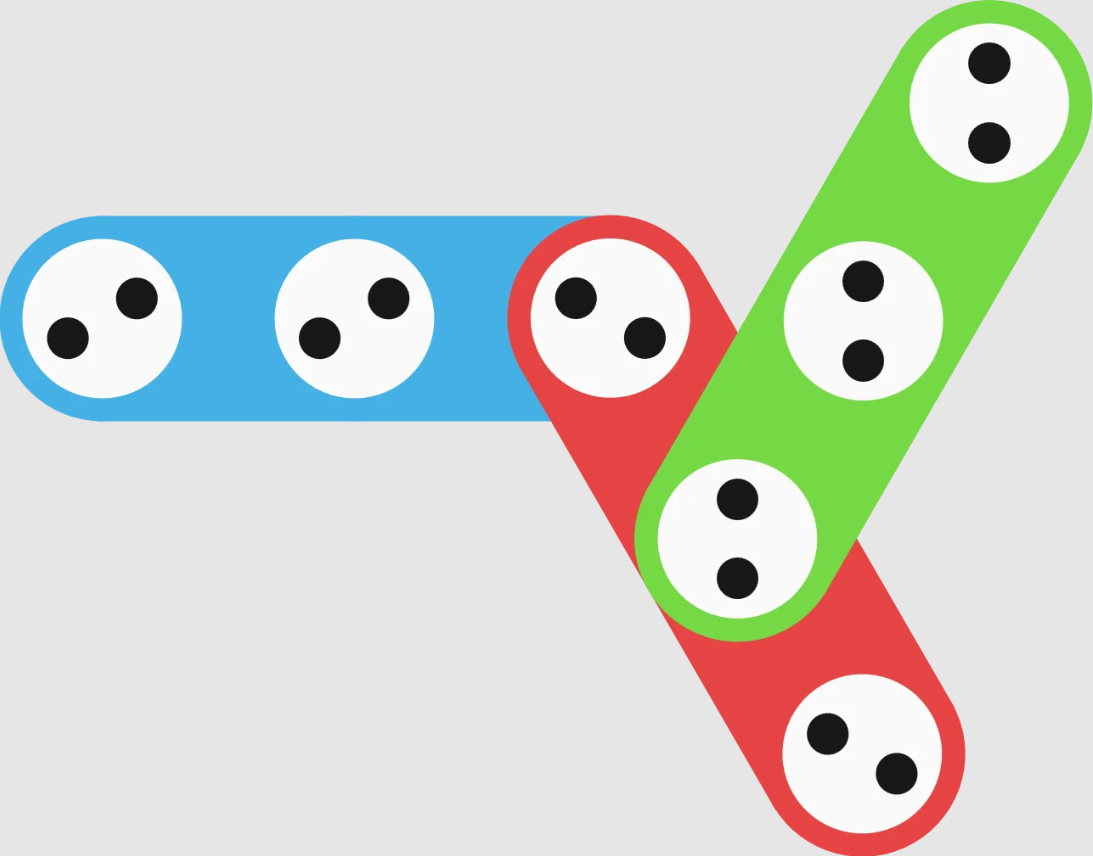
\includegraphics[width=0.5\textwidth]{Images/28076.png}
    \end{center}
\end{problem}

\section{연습문제 C}

\begin{problem}
    (8883번**) 주어진 다각형을 가로 $x_s$, 세로 $y_s$의 직사각형 종이 여러 개로 덮으려고 한다. 이때 종이의 각 변은 $x$축 또는 $y$축과 평행해야 하고 주어진 다각형의 회전은 불가능하다. 오차를 피하기 위해 지도가 종이의 바깥으로 $10^{-6}$까지 나가는 것을 허용한다. 필요한 종이의 수의 최솟값을 구하여라. 다각형의 꼭짓점의 수 $N$은 $3$ 이상 $50$ 이하의 정수이고 지도의 꼭짓점의 좌표 $(x, y)$는 $0 \leq x \leq 10x_s$와 $0 \leq y \leq 10y_x$를 만족한다.
\end{problem}

\begin{problem}
    (10069번*, IOI14) $0$부터 $M-1$까지 번호가 부여된 $M$개의 블록과 북쪽에는 서쪽 방향의 철도, 남쪽에는 동쪽 방향의 철도가 있는 길을 생각하자. 철도 사이의 블록 중 $N$개에는 $0$번부터 $N-1$번까지의 기차역이 하나씩 존재하며, 기차역이 있는 블록에는 북쪽 철로에서 남쪽 철로로 이어지는 세로 방향 철로 또는 남쪽 철로에서 북쪽 철로로 이어지는 세로 방향 철로가 있다. 또한 각 블록을 잇는 수평 방향 철로 사이에는 커넥터가 있다(회색 직사각형).
    
    \begin{center}
        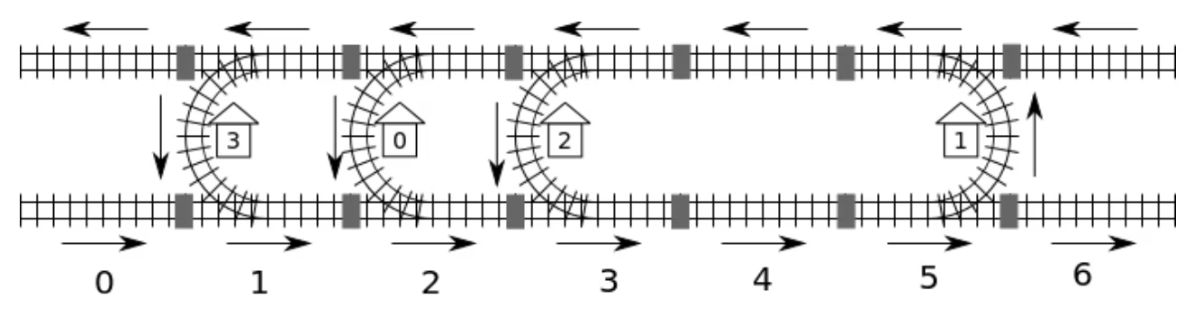
\includegraphics[width=0.8\textwidth]{Images/10069.png}
    \end{center}

    두 역 사이의 최단거리는 두 역 사이를 기차로 이동할 때 지나는 커넥터의 최소 개수이며, 모든 두 역 쌍에 대해 도달할 수 있음이 보장된다. 우리는 $0$번 기차역이 $C$번 블록 위에 있고 $0$번 기차역에 있는 철로의 방향이 북에서 남이라는 사실과 $Q$번의 두 역 사이의 최단거리에 대한 질의만으로 각 역이 있는 블록의 번호와 각 역에 있는 철로의 방향이 북에서 남인지, 남에서 북인지 알아내어야 한다.
    \begin{itemize}
        \item (서브테스크 1) $N \leq 100$이고 $Q$에 제한이 없으며, $0$번 역을 제외하면 나머지 역의 철로 방향은 남에서 북이다.
        \item (서브테스크 2) $N \leq 100$이고 $Q$에 제한이 없으며, $0$번 역의 오른쪽에 있는 철로 방향은 남에서 북이고, 왼쪽에 있는 철로 방향은 북에서 남이다.
        \item (서브테스크 3) $N \leq 5000$이고 $Q$는 $N(N-1)/2$ 이하여야 한다.
        \item (서브테스크 4) $N \leq 5000$이고 $Q$는 $3(N-1)$ 이하여야 한다.
    \end{itemize}

\end{problem}

\begin{problem}
    (10720번) 둘레의 길이가 $L$인 원형 레일을 $L$등분 한 후 각 지점에 $0$부터 $L-1$까지 번호를 붙였다. 그 위에 $N$마리의 시계 방향으로 이동하는 개미와 $M$마리의 반시계 방향으로 이동하는 개미가 있다. 모든 개미의 이동 속도는 초당 $1$이고, 개미는 충돌 이후 반대 방향으로 같은 속도로 이동하게 된다. 모든 개미가 처음과 같은 위치 및 이동 방향을 갖기 위해 필요한 시간 $T$를 출력하라. 단, 모든 개미는 구별되므로, 처음 그 자리에 있었던 개미가 다시 그 자리로 오는 때를 찾아야 한다. $L \leq 600$, $1 \leq N+M \leq 600$, $N \geq 1$, $M \geq 1$이다.
\end{problem}

\begin{problem}
    (15767번**) 이차원 좌표평면에 $N$개의 원이 있다. 다음 과정을 통해 원을 지워나간다.
    \begin{enumerate}
        \item 지워지지 않았고 반지름이 가장 큰 원들 중 인덱스가 가장 작은 원을 찾는다. 이 원을 \textit{target}이라 하자.
        \item \textit{target}과 겹치는 원을 모두 지운다. 겹친다는 것은 두 원의 내부 및 경계의 교집합이 공집합이 아님을 말한다.
    \end{enumerate}
    위 과정을 원이 모두 사라질 때까지 반복하면 각 원은 특정 반복에서 지워진다. 각 원이 지워진 반복에서 \textit{target} 원의 번호를 출력하는 프로그램을 작성하라. $N \leq 3 \cdot 10^5$이고 원의 중심 좌표는 절댓값이 $10^9$ 이하의 정수, 원의 반지름은 $10^9$ 이하의 자연수이다.
\end{problem}

\begin{problem}
    (18480번**) 겹치지 않는($r_i < l_{i+1}$) $N$개의 닫힌 구간 $[l_i, r_i]$의 합집합 $A$에 대해 크기가 $4$인 $A$의 부분집합들 중 합이 $s$인 부분집합의 개수를 구하여라. $N \leq 400$, $0 \leq s \leq 8 \times 10^8$, $0 \leq l_i \leq r_i \leq 2 \cdot 10^8$이다.
\end{problem}

\begin{problem}
    (18738번**) $1$부터 $2N$까지의 숫자가 정확히 한 번씩 적힌 $2N$장의 카드를 두 플레이어가 $N$장씩 나누어 갖는다. 그리고 다음과 같은 규칙으로 게임을 한다.
    \begin{itemize}
        \item 홀수번째 라운드에서는 선 플레이어가 먼저 카드를 내고, 짝수번째 라운드에서는 후 플레이어가 먼저 카드를 낸다.
        \item 각 라운드에서 두 번째로 카드를 내는 플레이어는 상대방이 낸 카드보다 큰 숫자가 적힌 카드를 1개 이상 갖고 있다면 그러한 카드(들) 중 하나를 내야 한다.
        \item 각 라운드에서 더 큰 숫자를 낸 플레이어가 그 라운드를 승리한다.
        \item 각 라운드에서 제출한 카드는 제거된다.
    \end{itemize}
    선 플레이어와 후 플레이어가 받은 $N$장의 카드가 각각 주어질 때, 선 플레이어가 이길 수 있는 라운드의 수의 최댓값을 구하여라. $N \leq 1000$이다.
\end{problem}

\newpage

\section{힌트}
\begin{hint}
    
\end{hint}
\begin{hint}
    정렬의 정의로 `모든 $i$와 $n>0$에 대해 $arr[i] < arr[i + n]$'를 사용하라.
\end{hint}
\begin{hint}
    Inversion Count가 무엇과 같다고 했었는지 생각해보라.
\end{hint}
\begin{hint}
    
\end{hint}
\begin{hint}
    
\end{hint}
\begin{hint}
    
\end{hint}
\begin{hint}
    
\end{hint}
\begin{hint}
    
\end{hint}
\begin{hint}
    
\end{hint}
\begin{hint}
    
\end{hint}
\begin{hint}
    
\end{hint}
\begin{hint}
    
\end{hint}
\begin{hint}
    
\end{hint}

\begin{hint}
    $N^2$ 알고리즘을 짜기에 $N$이 크다고 생각할 수 있지만, 단순 연산은 상수가 작아 시간 안에 돌기 충분하다.
\end{hint}

\begin{hint}
    기본적으로 케이스에 따라 분류해서 풀어야 하는데, 예외 케이스가 많아서 틀리기 쉽다. 그나마 쉬운 구현 방법은, 답이 무조건 31자리 이하 문자열임을 생각해서, 모든 31자리 이하 문자열들을 나열한 수열에서 $n/2+1$번째 문자열 바로 앞에 있는 문자열 $T$를 찾는다. 이렇게 하면, $n/2$번째 문자열과 같거나 더 사전순으로 뒤이고, $T$번째 문자열과 \textbf{같거나} 더 사전순으로 앞인 가장 짧은 문자열을 찾는 문제로 바뀐다. 그러면 생각할 예외 케이스가 크게 줄어든다.
\end{hint}

\begin{hint}
    두 개의 단계별 힌트가 있다.

    \textbf{[ 1 ]} \newline
    Inversion Count와 관련된 보존량을 생각해보자. 두 개씩 묶어서 이동시킬 때, Inversion Count의 ?는 항상 일정하다.

    \textbf{[ 2 ]} \newline
    보존량은 Inversion Count의 2로 나눈 나머지이다. 정렬된 배열에서 0이므로, 처음 배열의 Inversion Count가 홀수이면 불가능하다. 반면, 짝수일 때는 항상 가능하다. 짝수일 때 항상 가능하다는 것은 정렬할 수 있는 방법 하나만 제시하면 충분하다. 이는 직접 생각해보자.
\end{hint}

\begin{hint}
    $(a, b)$와 $(c, d)$를 마음대로 정할 수 있음에 주목하자. 일단, $(a, b)$, $(c, d)$와의 거리가 같은 점의 개수 조건을 무시하고 최대한 쉬운 직선을 그리자. 그리고 직선을 약간 회전시키면, 개수 조건을 만족시키게 할 수 있다!
\end{hint}

\begin{hint}
    두 개의 단계별 힌트가 있다.

    \textbf{[ 1 ]} \newline
    $i$번째에 있는 어떤 수 $k$가 첫 번째에 오게 하려면 $[1, i]$에 모두 $k$보다 크거나 작은 수가 있어야 한다. 이것은 제일 처음에 `1 $N$ I' 연산을 써서 $1, 2, 3, \cdots, N$으로 정렬시키면 만족시킬 수 있다. `1 $k$ D' 연산을 쓰면 내림차순 정렬된다. 

    \textbf{[ 2 ]} \newline
    첫 번째 수는 결정되었으므로, 두 번째 수를 같은 방법으로 결정한다. 그런데, `2 $N$ I' 연산을 써서 다시 정렬시킨다면 $N$번 이하의 연산으로 수행할 수 없을 것이다. 중요한 것은, 처음 정렬을 했기 때문에 여전히 $[2, i]$에 모두 $k$보다 크거나 작은 수가 있다는 조건이 유지된다는 것이다. 왜 그런지는 스스로 고민해보자.
\end{hint}

\begin{hint}
    세 개의 단계별 힌트가 있다.

    \textbf{[ 1 ]} \newline
    $K$가 정렬된 배열에서 $i$번째 수와 $i+1$번째 수의 차이의 최댓값이면 항상 정렬 가능하다. 정렬된 배열에서 $a$번째에 해당하는 수와 정렬된 배열에서 $b(>a)$번째에 해당하는 수를 바꾸려면, $a$와 $a+1$번째를 위치를 바꾸고, $a+1$번째와 $a+2$번째를 바꾸고, ... 을 반복하면 되기 때문이다.

    \textbf{[ 2 ]} \newline
    하지만, 배열 자체가 굳이 교환이 필요없는 고립된 몇 개의 구간으로 나눠진다면 어떨까? $2, 1, 102, 101$ 순으로 나열된 배열에서 $2$와 $101$은 바꿀 필요가 없기 때문에 답은 $99$가 아닌 $1$이 된다. 여기서 $2, 1$과 $102, 101$은 두 구간 사이에서 교환이 필요없는 고립된 구간이다.

    \textbf{[ 3 ]} \newline
    고립된 구간은 정렬된 배열의 각 수의 원래 위치를 알면 쉽게 찾을 수 있다. 이것은 $1, 2, \cdots, N$이 섞인 순열(permutation)으로 나올텐데, 순열에서 원래 그 구간에 속한 값들끼리만 서로 섞이게 된다. 예를 들어 $\cdots, 6, 7, 8, 5, \cdots$와 같이 있다면, $6, 7, 8, 5$($5, 6, 7, 8$)는 고립된 구간이다.
\end{hint}

\begin{hint}
    두 개의 단계별 힌트가 있다.

    \textbf{[ 1 ]} \newline
    동치 관계(equivalence relation)를 생각하자. 정의와 성질을 모르는 사람들은 아래의 설명을 참고하라.
    
    이항 관계는 어떤 집합 $S$에 대해 $\{(x, y)~|~x \in S, y \in S\}$의 부분집합인 $R$을 말한다. 이항 관계 중에서 다음 세 조건을 만족하는 관계를 특별히 동치 관계라고 한다.
    \begin{enumerate}
        \item $(i, i) \in R$
        \item $(i, j) \in R$이면 $(j, i) \in R$
        \item $(i, j) \in R$이고 $(j, k) \in R$이면 $(i, k) \in R$
    \end{enumerate}
    동치 관계가 $R$에 대해서, 집합 $S$를 동치 관계가 성립하는 것끼리 분할할 수 있다. 즉, $S_1 \cup S_2 \cup \cdots \cup S_p = S$이면서 $S_i \cap S_j = \phi ~ (i \neq j)$이게 $S$를 분할하면서, $S_i$에 속하는 임의의 두 원소 사이에 동치 관계가 성립하고, $S_i$에 속하는 임의의 원소와 $S_j ~ (i \neq j)$에 속하는 임의의 원소 사이에 동치 관계가 성립하지 않게 할 수 있다.

    \textbf{[ 2 ]} \newline
    $i$번째 수와 $j$번째 수를 바꿀 수 있을 때 $(i, j)$를 $R$에 포함시키면, $R$은 $S = \{1, 2, \cdots, n\}$에 대한 이항 관계 중에서 동치 관계가 된다. 즉, $A_i$와 $A_j$를 바꿀 수 있다는 것과 $(i, j) \in R$은 동치이다. 그리고, 결국 정렬된 배열 $B$에 대해 $A_i$ 위치에 $B_i$가 와야 한다.
\end{hint}

\begin{hint}
    멀티탭이 꽂히는 순서를 $3$으로 나눈 나머지가 다른 두 멀티탭은 하나가 다른 하나에 완전히 포함될 수 없다. 이에 착안하면 정확히 세 개의 멀티탭만 제일 위에 보이게 할 수 있고, 이 경우가 최적이다.
\end{hint}

\begin{hint}
    \url{https://icpcarchive.github.io/World%20Finals/ICPC%20World%20Finals/2013%20ICPC%20World%20Finals/solution.pdf}
\end{hint}

\begin{hint}
    \url{https://blog.myungwoo.kr/46}
\end{hint}

\begin{hint}
    처음 개미에 임의로 번호를 부여한다. 그러면 두 개미간의 충돌은, 스쳐 지나가면서 서로의 번호를 교환하는 것과 같다. 답이 $L \cdot (N+M)$ 이하임이 보장되고 충돌은 $L$초를 주기로 돌아오기 때문에, 충돌하는 시각을 모두 기록하고 단순 시뮬레이션하면 $O(L \cdot (N+M)^2)$에 구현할 수 있다.
\end{hint}

\begin{hint}
    \url{https://jjang36524.tistory.com/26}
\end{hint}

\begin{hint}
    네 개의 단계별 힌트가 있다.

    \textbf{[ 1 ]}
    자주 쓰이는 트릭으로 다항식을 활용하는 방법이 있다. 어떤 수 $a$를 뽑는 것을, 다항식에서 $x^a$을 선택하는 것으로 바꾸면, 합이 $s$가 되게 하는 경우의 수는 다항식들을 곱한 다항식에서 $x^s$의 계수가 된다.

    \textbf{[ 2 ]}
    집합을 고르는 것이므로 같은 수의 선택은 불가하고 고르는 순서는 중요하지 않다. 따라서, $A(x) = \sum_{1 \leq i \leq n} {\left(x^{l_i} + x^{l_i+1} + \cdots + x^{r_i}\right)}$라 두고 포함과 배제의 정리를 사용하자.

    \textbf{[ 3 ]}
    전체 경우를 $(a, b, c, d)$와 같이 전부 다른 경우, $(a, a, b, c)$와 같이 정확히 두 개만 같은 경우, $(a, a, b, b)$로 두 개씩 같은 경우, $(a, a, a, b)$로 세 개만 같은 경우, $(a, a, a, a)$로 네 개 다 같은 경우로 나누자. 즉,
    $$A(x)^4 = (a, b, c, d) + (a, a, b, c) + (a, a, b, b) + (a, a, a, b) + (a, a, a, a)$$
    가 된다. 이제 각각을 구하자.
    
    \begin{itemize}
        \item $(a, a, a, a)$ : 같은 수를 정확히 네 개 선택하는 것은 $A(x^4)$으로 쓸 수 있다. 즉, $A(x^4)$과 같다.
        \item $(a, a, a, b)$ : $a=b$인 경우를 무시하면 같은 수를 정확히 세 개 선택하고, 어떤 수를 한 번 선택하는 것은 $A(x^3)A(x)$가 된다. 그런데, $a=b$인 항은 $A(x^4)$으로 쓸 수 있고 $a \neq b$인 항은 지수가 달라 한 번씩 나타나므로, $A(x^3)A(x) - A(x^4)$가 된다. 순서를 바꾸는 방법의 수 $\frac{4!}{3!} = 4$를 곱하면 $(a, a, a, b)$가 나온다.
        \item $(a, a, b, b)$ : $a=b$인 경우를 무시하면, 같은 수를 정확히 두 개 선택하는 것을 두 번 반복하는 것은 $A(x^2)A(x^2)$가 된다. 그런데, $a=b$인 항은 $A(x^4)$이고, $a \neq b$인 항은 지수가 같아 두 번씩 나타나므로, $\frac{1}{2}\left[A(x^2)^2 - A(x^4)\right]$이 된다. 순서를 바꾸는 방법의 수 $\frac{4!}{2!2!} = 6$을 곱하면 $(a, a, b, b)$가 나온다.
        \item $(a, a, b, c)$ : $a, b, c$가 모두 달라야 한다는 조건을 무시하면 $A(x^2)A(x)A(x)$가 된다. 여기서 $b \neq c$를 적용하면 위와 같은 방식으로 $\frac{1}{2} A(x^2) \left[ A(x)^2 - A(x^2) \right]$가 된다. 이제 $a \neq b$와 $a \neq c$를 생각하면, $(a, a, a, b)$에서 구했던 항인 $A(x^3)A(x) - A(x^4)$을 추가로 빼면 된다. 이렇게 구한 항에 순서를 바꾸는 방법의 수 $\frac{4!}{2!} = 12$를 곱하면 $(a, a, b, c)$가 나온다.
    \end{itemize}

    이렇게 구한 $(a, b, c, d)$를 $4!=24$로 나누면 원하는 답이 된다. 즉,
    $$\frac{1}{24}\left[A(x)^4 - 6A(x^2)A(x)^2 + 3A(x^2)^2 + 8A(x^3)A(x) - 6A(x^4)\right]$$
    이다.

    \textbf{[ 4 ]}
    \textbf{[ 3 ]}의 식에서 뒤 네 개의 항은 $A(x) = \sum_{1 \leq i \leq n} {\left(\frac{x^{r_i+1} - x^{l_i}}{x-1}\right)}$로 두면 항의 개수가 $2n$개인 다항식 세 개의 곱셈이므로 $O(n^3)$에 답을 구할 수 있다. 나눗셈은 $x^k-1$ 꼴의 다항식으로 나누는 것만 처리하면 되고, 나누어 떨어짐이 보장되므로, 곱셈 공식을 이용해 해결할 수 있다.

    제일 앞 항은 meet in the middle로 해결한다. 먼저, $x^k$을 $(x-1)^4$으로 나눈 몫은 $\binom{3}{3} \cdot x^{k-4} + \binom{4}{3} \cdot x^{k-5} + \cdots$로 표현되기 때문에, $A(x)^4$에 포함된 $c \cdot x^k$에 대해 $c \cdot \binom{k-1-s}{3}$을 다 더하면 된다. 이것을 meet in the middle로 해결하려면 $A(x)^2$에 포함된 $c \cdot x^k$와 $A(x)^2$의 곱인 다항식에서 답을 구하고, $k$를 증가시키며 빠른 시간이 이 값을 업데이트해야 한다. 이것은 
    $$\binom{a+b}{k} = \sum_{i=0}^k {\binom{a}{i}\binom{b}{k-i}}$$
    을 이용하여 해결할 수 있다. $A(x)^2 = \sum d \cdot x^l$로 쓰면, 빠르게 업데이트해야 하는 값은 $T_3 = \sum d \cdot \binom{k+l-1-s}{3}$가 되는데, 위 식을 사용하면 $T_2 = \sum d \cdot \binom{k+l-1-s}{2}$, $T_1 = \sum d \cdot \binom{k+l-1-s}{1}$, $T_0 = \sum d \cdot \binom{k+l-1-s}{0}$와 $k$의 증가량을 $\Delta k$에 대한 식으로 $O(1)$의 시간에 $T_3, T_2, T_1, T_0$ 모두 업데이트 할 수 있게 된다.
\end{hint}

\begin{hint}
    \url{https://qoj.ac/contest/446/problem/1441/statistics}
\end{hint}